\graphicspath{{general_design/fig/}}

\chapter{Design}
\label{chap:general_design}

\begin{figure}[!h]
    \centering
    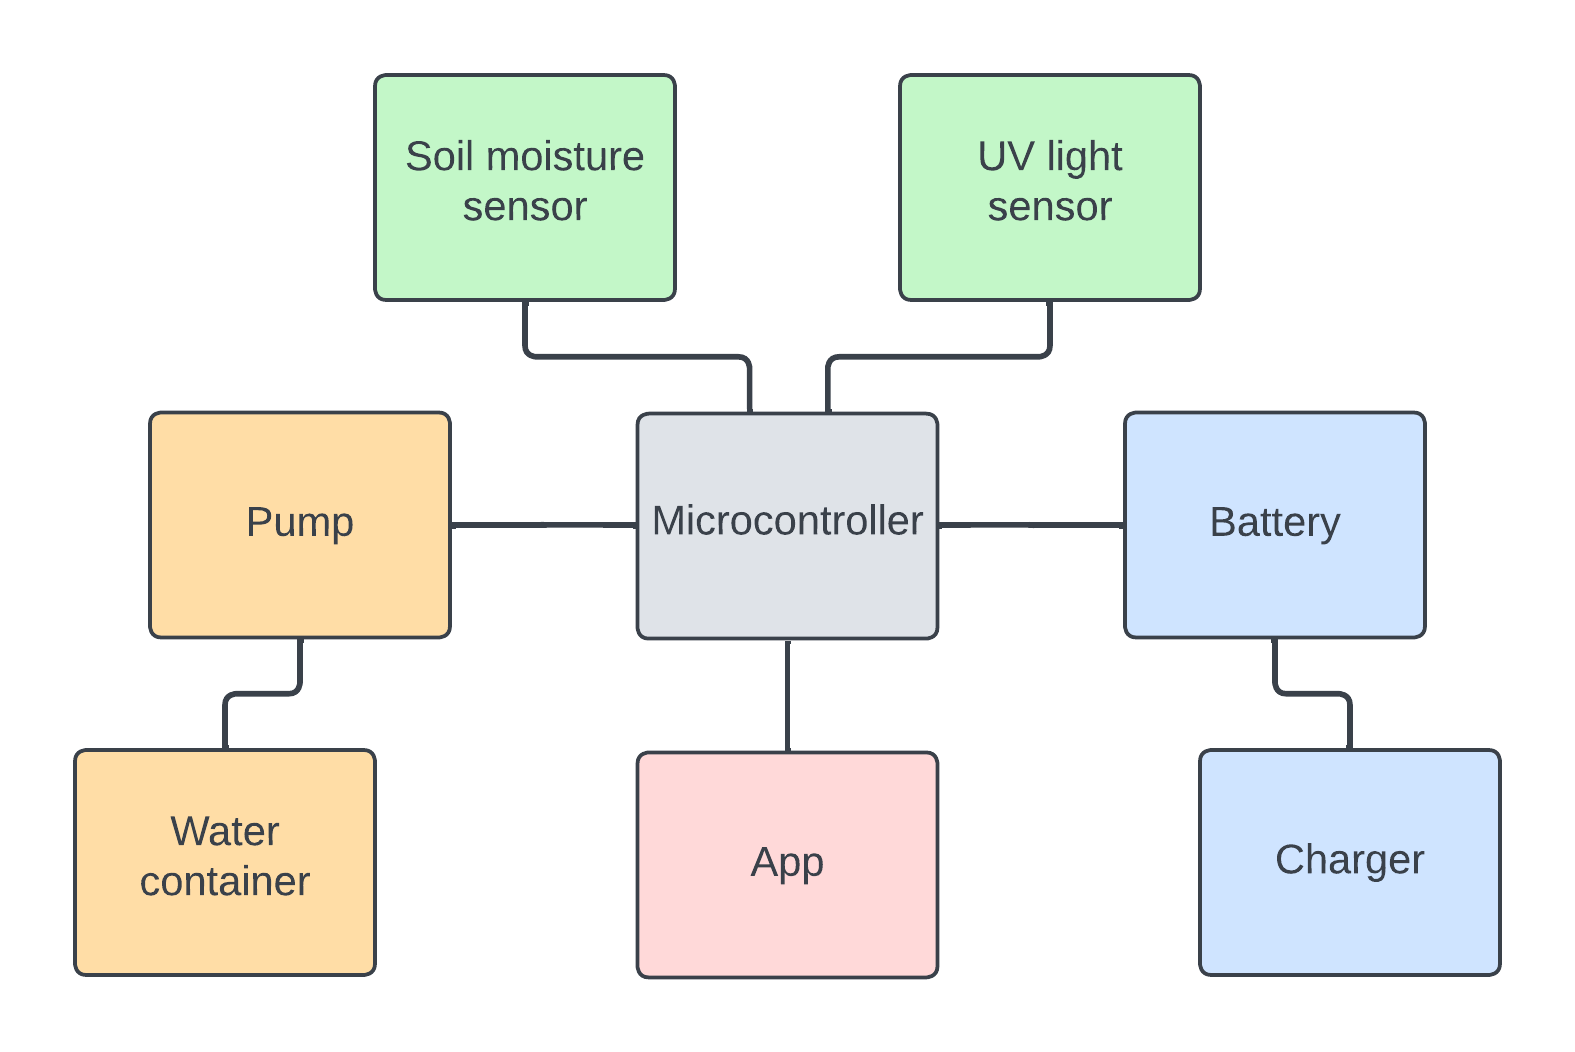
\includegraphics{design_diagram.png}
    \caption{Design overview}
    \label{fig:design_overview}
\end{figure}

Data from a soil moisture and UV light sensor will be monitored using a microcontroller. When soil moisture levels fall below a set value, a pump will turn on to water the plant until the soil reaches the target moisture level. The soil moisture, UV light exposure and watering times will be logged by the microcontroller and sent to an app. The user can use the app to view the data and set the moisture level target. The system will be powered by a battery that charges when power is available.
%%%%%%%%%%%%%%%%%%%%%%%%%%%%%%%%%%%%%%%%
\section{Microcontroller}
The ESP32-C3-DevKitC-02 will be used for this project as it is WiFi and Bluetooth capable.

%%%%%%%%%%%%%%%%%%%%%%%%%%%%%%%%%%%%%%%%
\section{UV light and soil moisture sensing}
A capacitive soil moisture sensor will be used as they do not rust like resistive sensors would. Both the soil moisture sensor and UV light sensor can be connected to a microcontroller without any additional circuits. The soil moisture sensor outputs a measurement equivalent voltage, while the UV light sensor communicates using I2C.

%%%%%%%%%%%%%%%%%%%%%%%%%%%%%%%%%%%%%%%%
\section{Automatic watering}
The pump will be controlled by the microcontroller and powered by the battery. A drive circuit needs to be added to ensure the pump receives the correct voltage and current. A peristaltic pump will need to be used to prevent siphoning. Siphoning can also be prevented by using valves along with a small centrifugal pump. A peristaltic pump will be used to keep the final device as compact as possible. 

%%%%%%%%%%%%%%%%%%%%%%%%%%%%%%%%%%%%%%%%
\section{App}
The app will allow the user to view the UV light exposure, soil moisture levels and watering over time. The app will also allow the user to connect the microcontroller to WiFi and set the target soil moisture level. 

%%%%%%%%%%%%%%%%%%%%%%%%%%%%%%%%%%%%%%%%
\section{Battery and charging}
The battery will need to be able to power the system for at least two hours at a time. This is to ensure the system functions during loadshedding. The battery needs to be charged whenever power is available. A charging circuit will need to be designed.


%%%%%%%%%%%%%%%%%%%%%%%%%%%%%%%%%%%%%%%%
\section{PCB}
To keep the final system as compact as possible, a PCB will be designed for the circuits.

%%%%%%%%%%%%%%%%%%%%%%%%%%%%%%%%%%%%%%%%
\section{Case}
The final system will be contained in a compact, durable case.